%\vspace{-0.1in}
\section{Introduction}
\label{sec:intro}

Public cloud providers like Microsoft~\cite{dcqcn} and Google~\cite{timely} are
deploying RoCE in their data centers to enable low latency, high throughput data
transfers with minimal CPU overhead~\cite{dcqcn}. Systems like
Pilaf~\cite{pilaf}, Farm~\cite{farm}, TesnorFlow~\cite{tensorflow}, and
CNTK~\cite{cntk} rely on RoCE for enhanced performance.

RoCE uses Priority Flow Control (PFC) to prevent packet drops due to buffer
overflow at the switches. PFC allows a switch to temporarily pause its upstream
neighbor. While PFC is effective, it can lead to
deadlocks~\cite{rdmaatscale,tcpbolt,hu2016deadlocks}.

Deadlocks in PFC-enabled network are caused by circular buffer dependency
(CBD)~\cite{hu2016deadlocks}. Figure~\ref{fig:deadlock_example} illustrates a
3-node CBD: switch A is blocked by switch B, which is blocked by C, which is
blocked by A.

The deadlock problem is not merely theoretical -- our conversations with
engineers at large cloud providers confirm that they have seen the problem in
practice and at least one provider has reported it publicly~\cite{rdmaatscale}.
Deadlock is a serious problem because a deadlock is not transient -- once a
deadlock forms, it does not go away even after the conditions (e.g. a temporary
routing loop due to link failure) that caused its formation have
abated~\cite{rdmaatscale}. Worse, a small initial deadlock may cause the PFC
frames to propagate and create a global deadlock, and shutdown the whole
network.

Current solutions to the deadlock problem fall in two categories. The first
category consists of solutions that {\em detect} the formation of the deadlock
and then use various techniques to {\em break} it~\cite{shpiner2016unlocking}.
These solutions do not address the root cause of the problem, and hence cannot
guarantee that the deadlock would not immediately reappear.

The second category of solutions are designed to {\em prevent} deadlocks.  For
deadlock formation, CBD is {\em necessary}, but not {\em
sufficient}~\cite{hu2016deadlocks}. Unfortunately, {\em sufficient} conditions
for deadlock formation are not well understood~\cite{hu2016deadlocks}. Thus,
currently, preventing CBD is the only practical way to prevent deadlocks.

In \S\ref{sec:challenges}, using data from a large cloud provider's data
centers, we show that any practical deadlock prevention scheme must meet three
key challenges. These include: $(i)$ it should require no changes to existing
routing protocols or switch hardware, $(ii)$ it must deal with link failures and
associated  route changes, and $(iii)$ it must work with limited buffer
available in commodity switches.

While a number of schemes for preventing deadlocks have been proposed, they fail
to meet one or more of these challenges.  Some schemes require centralized,
SDN-style routing.  These are difficult to deploy in existing data centers,
without wholesale infrastructure changes.  Others are distributed, but brand-new
routing protocols~\cite{tcpbolt} that are not supported by commodity switches.
Many of these schemes also require carefully controlling the paths -- something
that is simply not possible with decentralized routing in presence of link
failures~\cite{netpilot}.  Finally, some schemes require creation of numerous
priorities and buffer management according to those priorities. For example, if
each of the flows in Figure~\ref{fig:deadlock_example} had its own priority and
was buffered separately at each switch, there would be no deadlock.  However,
modern data center networks, built using commodity switches, can realistically
support only two or three lossless priorities~\cite{rdmaatscale}.  Thus, to the
best of our knowledge, no deadlock free routing solution has been deployed in a
production data center.  

In this paper, we present \sysname{}, which meets all three challenges described
above. \system is based on a simple observation: in a data center, we can ask
the operator to supply a list of paths that the operator wants to be lossless.
We call these expected lossless paths (ELPs). Enumerating ELPs is
straightforward for ``structured'' topologies like Clos~\cite{clos},
FatTree~\cite{fattree} and Bcube~\cite{bcube}, and not onerous even for
randomized topologies like Jellyfish~\cite{jellyfish}. 

Using ELPs, we create a system of match-action rules to ``tag'' packets. The
switches use these tags to enqueue packets in different lossless queues. The tag
values are such that CBD never forms due to packets travelling on paths in ELP.
If packets ever deviate from paths in ELP (e.g. due to link failures or routing
errors) they are automatically placed in a lossy queue to ensure that they do
not trigger PFC. \system guarantees that there will be no deadlock - even under
unforeseen link failures or routing errors. Even routing loops won't lead to
deadlock!

\system works for any routing protocol. There are no restrictions on what paths
can be included in the ELP. Tagging rules are completely static and are
specified only in terms of local information (tag, ingress port and egress port)
available at each switch. 

The number of lossless queues and the number of tag match-action rules are
small.  Even for a Jellyfish topology with 2000 switches, \sysname{} requires
just three lossless queues per switch.  In fact, we prove that for Clos
topology,  \sysname{} is optimal in terms of number of lossless queues required.
We also show how to minimize the number of match-action rules required to
implement \sysname{}.

We have implemented and tested \sysname{} on commodity Arista 7050 Switches with
Broadcom chipsets. The implementation requires carefully addressing the problem
of priority transition (\S\ref{sec:implementation}). Our tests show that
\sysname{} has no performance penalty on datapath.

\begin{figure}
	\centering
	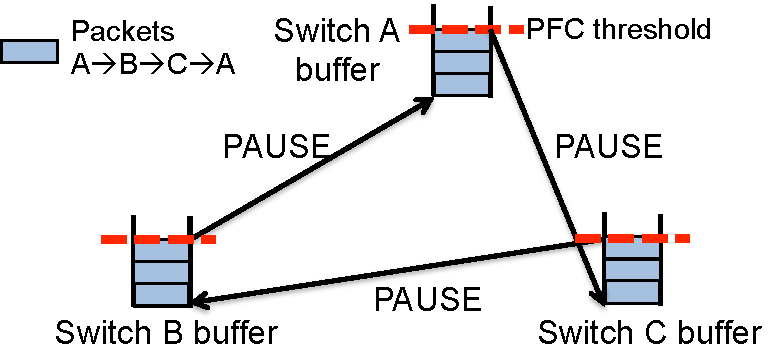
\includegraphics[width=0.5\textwidth] {figs/deadlock}
	\vspace{-0.15in}
	\caption{PFC-induced deadlock: simple illustration of CBD.}
	\vspace{-0.15in}
	\label{fig:deadlock_example}
\end{figure}
